\documentclass[11pt]{article}

\usepackage[margin=1in]{geometry}
\usepackage{amsmath,amssymb}
\usepackage{booktabs}
\usepackage{graphicx}
\usepackage{tabularx}
\usepackage{microtype}

\title{Result 3.\\
Hydrodynamic entropy of GraphCast:\\
squared processor-edge output on the real mesh lengths}
\author{}
\date{}

\begin{document}
\maketitle

\section{What is being measured}

Result 1 assigns an energy to each mesh length from the mesh-edge encoder. Result 2 assigns one from the spherical-harmonic power of the latent field on the nodes. This result uses the same energy as Result 1, on the vectors the processor writes onto the edges.

GraphCast Small is run for one forecast step. Each of the 16 processor steps has its own edge network. The input of an edge is the sender node's latent, the edge's own embedding, and the receiver node's latent, concatenated. The network writes a \(512\)-vector on that edge. The energy of level \(m\) at step \(s\) is the mean, over the edges labeled \(m\), of the squared Euclidean norm of that vector:
\[
E_s(m) = \mathrm{mean}_{e \in M_m}\,\|\mathbf{y}_{s,e}\|^2.
\]
The residual that GraphCast then adds back onto the edge is not included. \(\mathbf{y}_{s,e}\) is the output of that step's edge network, after its layer norm.

The entropy is the same formula as in Result 1,
\[
p_i = \frac{E_i}{\sum_j E_j},
\qquad
H = -\sum_i p_i \ln p_i,
\qquad
H_n = \frac{H}{\ln N}.
\]
\(H\) is in nats. Six levels give \(\ln 6 = 1.792\). The wavenumber is \(k = 1/L(m)\), with
\[
L(m) = \frac{\pi R}{2 \cdot 2^{m}}, \qquad R = 6371\,\mathrm{km},
\]
from \(10008\,\mathrm{km}\) at \(M_0\) to \(313\,\mathrm{km}\) at \(M_5\).

\section{Procedure}

The run uses the published GraphCast Small checkpoint: \(1.0^\circ\), 13 pressure levels, mesh size 5, latent size 512, 16 processor steps. Nothing is retrained. The input is the published ERA5 state for 2022-01-01 at \(1.0^\circ\) with 13 pressure levels, normalized with the checkpoint's own per-level mean and standard deviation. The target is the atmosphere six hours later. This is the same forecast as Result 2. The decoded 2\,m temperature has global mean \(276.9\,\mathrm{K}\).

An edge is labeled by the split that created it, using the same face-to-edge order as the mesh graph. The counts are \(60\), \(240\), \(960\), \(3840\), \(15360\), and \(61440\). The row labeled encoder is the mesh-edge embedding written before the first processor step. The rows labeled \(1\) through \(16\) are the edge-network outputs of those processor steps.

\section{Results}

\begin{center}
\begin{tabular}{lrrrr}
\toprule
Step & \(H\) (nats) & \(H_n\) & slope & share on \(M_0\) \\
\midrule
Encoder & 1.678 & 0.937 & \(-0.451\) & 19.4\% \\
1 & 1.748 & 0.976 & \(-0.163\) & 27.8\% \\
2 & 1.756 & 0.980 & \(-0.141\) & 26.7\% \\
3 & 1.788 & 0.998 & \(-0.046\) & 20.0\% \\
4 & 1.738 & 0.970 & \(-0.087\) & 25.6\% \\
5 & 1.737 & 0.969 & \(-0.192\) & 24.5\% \\
6 & 1.730 & 0.965 & \(-0.183\) & 25.9\% \\
7 & 1.782 & 0.994 & \(-0.057\) & 18.4\% \\
8 & 1.765 & 0.985 & \(+0.084\) & 14.2\% \\
9 & 1.787 & 0.997 & \(+0.005\) & 15.2\% \\
10 & 1.777 & 0.992 & \(-0.132\) & 18.7\% \\
11 & 1.767 & 0.986 & \(-0.164\) & 19.3\% \\
12 & 1.784 & 0.996 & \(+0.076\) & 15.6\% \\
13 & 1.684 & 0.940 & \(+0.214\) & 13.3\% \\
14 & 1.705 & 0.952 & \(+0.188\) & 14.2\% \\
15 & 1.613 & 0.900 & \(+0.293\) & 11.4\% \\
16 & 1.577 & 0.880 & \(+0.280\) & 11.7\% \\
\bottomrule
\end{tabular}
\end{center}

The power-law fit is weak. The coefficient of determination is \(0.59\) at the encoder, \(0.22\) at step 8, and \(0.40\) at step 16. From step 8 onward the fitted slope is positive at most steps: the finest edges carry more squared output than the coarsest. At step 16 the six energies are \(7.08\), \(6.59\), \(6.40\), \(6.39\), \(6.85\), and \(26.96\), so \(M_5\) holds the largest share and \(M_0\) holds \(11.7\%\).

\begin{figure}[ht]
\centering
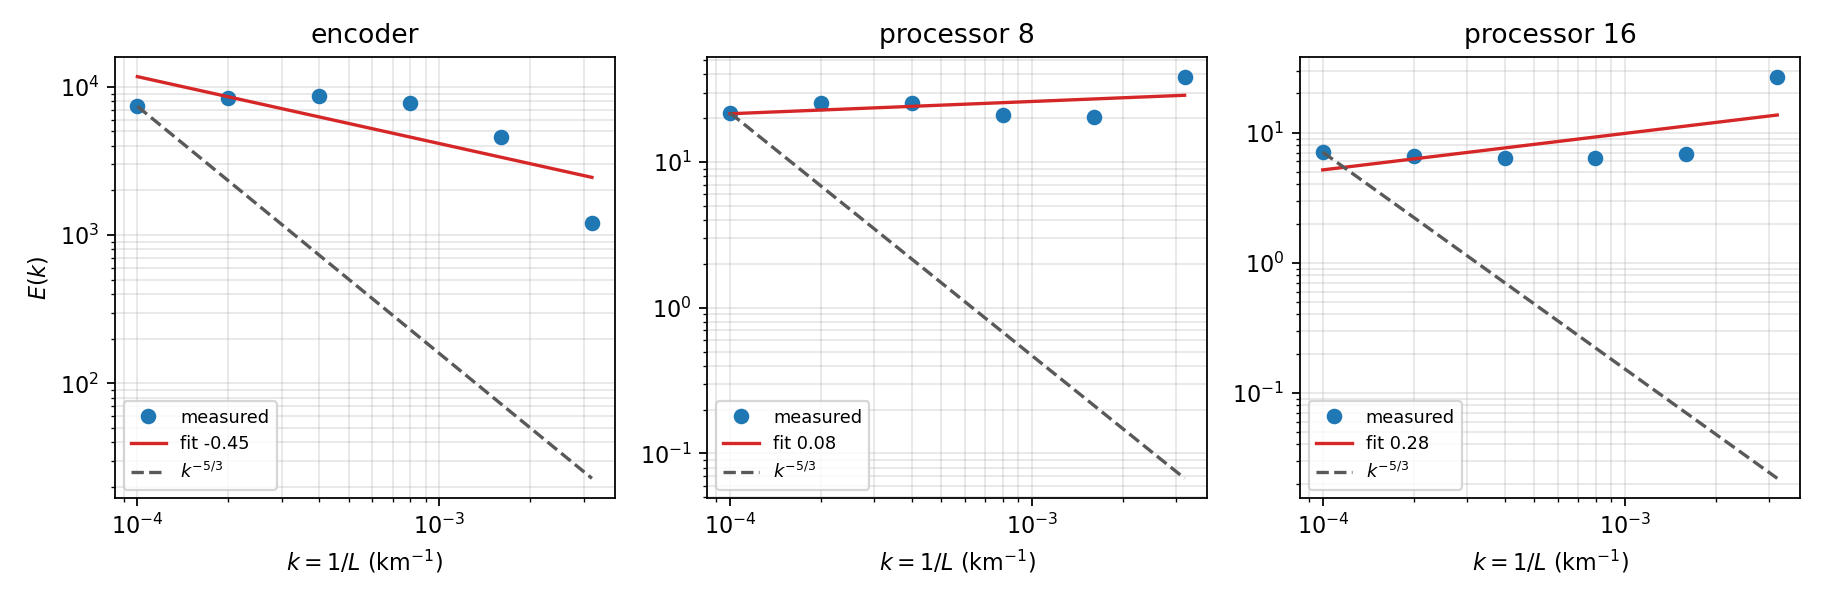
\includegraphics[width=\textwidth]{outputs/graphcast_processor_edge_entropy.png}
\caption{Energy against \(k = 1/L\) for the encoder embedding and for processor steps 8 and 16. Circles are the measured mean squared edge output. The solid line is the power-law fit of that panel. The dashed line is \(k^{-5/3}\), drawn through that panel's own \(M_0\) energy. Absolute height is not comparable across panels.}
\end{figure}

\section{Comparison with Result 1 and the local baseline}

\noindent
\begin{tabularx}{\textwidth}{@{}lXXX@{}}
\toprule
& Local notebooks & Result 1, after layer norm & This calculation \\
\midrule
Input
  & Edge geometry only
  & Edge geometry only
  & ERA5 state, one forecast step \\
Vector
  & \(\|W_0\mathbf{x}+\mathbf{b}_0\|^2\)
  & Encoder output after layer norm
  & Processor edge output after its layer norm \\
Levels
  & \(M_0\)--\(M_5\)
  & \(M_0\)--\(M_5\)
  & The same six lengths \\
\bottomrule
\end{tabularx}

\begin{center}
\begin{tabular}{lrrrr}
\toprule
& \(H\) (nats) & \(H_n\) & slope & share on \(M_0\) \\
\midrule
Local \texttt{linear\_0} & 0.835 & 0.466 & \(-1.866\) & 70.5\% \\
Result 1, after layer norm & 1.789 & 0.998 & \(-0.061\) & 17.8\% \\
This run, encoder & 1.678 & 0.937 & \(-0.451\) & 19.4\% \\
This run, step 16 & 1.577 & 0.880 & \(+0.280\) & 11.7\% \\
\bottomrule
\end{tabular}
\end{center}

The local value \(0.835\) nats is the geometric scaling of \(\|\mathbf{x}\|^2\) with edge length, and its slope sits near \(-2\). The processor outputs do not. Each of those networks ends in a layer norm, which divides out the magnitude of the \(512\)-vector, and the magnitude is where the edge length would have entered. What remains is a shallow spectrum. \(H_n\) stays between \(0.880\) and \(0.998\) at every step, against an equal-share value of \(1\). The dashed \(k^{-5/3}\) line, whose slope is \(-1.67\), falls away from the measured points in every panel.

The encoder row of this run is not a replay of Result 1. Result 1 fed each edge \((\Delta x, \Delta y, \Delta z, \|\Delta\|)\) in the global frame. During the forecast the same encoder weights are fed the spatial features GraphCast builds for the edge, with the receiver position taken relative to the sender. The weights match. The \(4\)-vector does not, so the embedding differs: \(H = 1.678\) nats here and \(1.789\) nats in Result 1. The \(276.9\,\mathrm{K}\) temperature check is what ties this run to the same forecast as Result 2.

\end{document}
